
%% Refer to latex document when possible
\pdfoutput=1
\documentclass[10pt]{beamer}

%STANDARD PREAMBLE
%https://tex.stackexchange.com/questions/68821/is-it-possible-to-create-a-latex-preamble-header
\usepackage{/Users/mwojno01/Research/LabMeetings/beamer_preamble}


\title{Why Bayes}
%\subtitle{}

\begin{document}

\maketitle

%
%\begin{frame}{Underlying goals}
%
%This lightning chat is motivated by the following goals:
%
%\begin{enumerate}
%\item Demonstrate how to make Bayesian inference fast and easy for Bayesian logistic regression (and associated models).
%\item Exemplify the ``augmentation trick". 
%\item Reinforce knowledge of routine Bayesian regression-type calculations. 
%\end{enumerate}
%\end{frame}
%
%\begin{frame}{Table of contents}
%  \setbeamertemplate{section in toc}[sections numbered]
%  \setbeamertemplate{subsection in toc}[subsections numbered]
%   \setbeamertemplate{subsection in toc}{\leavevmode\leftskip=3.2em\rlap{\hskip-2em\inserttocsectionnumber.\inserttocsubsectionnumber}\inserttocsubsection\par} %indents the subsections
%  \tableofcontents%[hideallsubsections]
%  %\setcounter{tocdepth}{3} 
%\end{frame}

\section{Why Bayes?}
\subsection{Estimating the probability of a rare event}

\begin{frame}{Description of problem}
\red{TODO}
\end{frame}

\begin{frame}{From prior to posterior}

\begin{center}
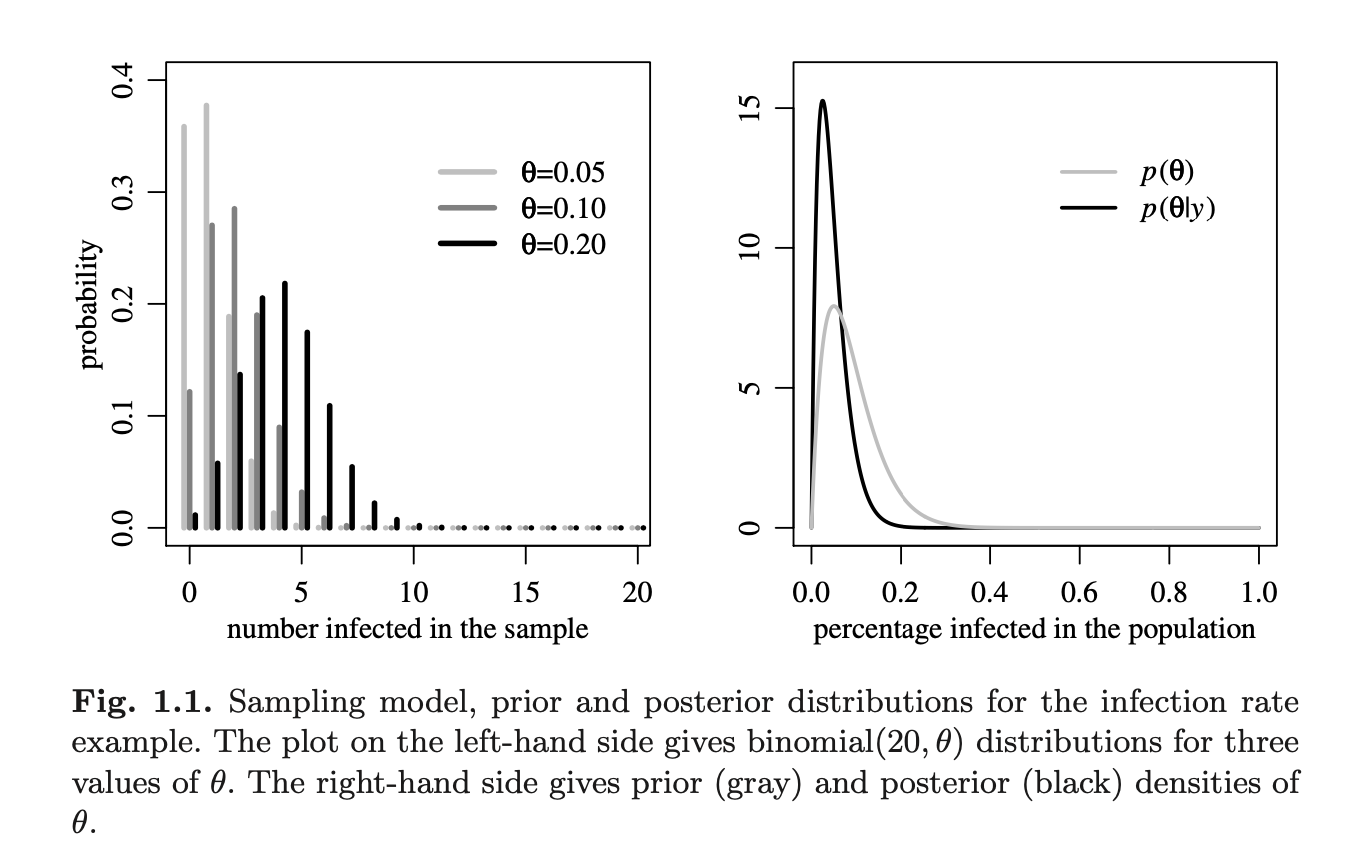
\includegraphics[width=.75\textwidth]{images/hoff_fig1dot1_prior_posterior_shift}
\end{center}

\scriptsize
\begin{minipage}{.45\textwidth}

\begin{align*}
\textbf{Prior} & \\
\theta  \sim  \Beta(2,20)   &\\ 
\E[\theta]  = 0.09 &\\
\text{mode}[\theta] =0.05 &\\
P(\theta < 0.10) = 0.64 &\\
P(0.05 < \theta < 0.20) = 0.66&  \\
\end{align*}

\end{minipage} \hfill
\begin{minipage}{.45\textwidth}

\begin{align*}
\textbf{Posterior} & \\
\theta \cond \set{Y=0}  \sim  \Beta(4,20)  &  \\ 
\E[\theta \cond \set{Y=0}  ] = 0.048& \\
\text{mode}[\theta \cond \set{Y=0}  ] =0.025& \\
P(\theta < 0.10 \cond \set{Y=0} ) = 0.93 &\\
\end{align*}

\end{minipage}


\end{frame}


\end{document}



